\begin{figure}[!ht]
	\centering
	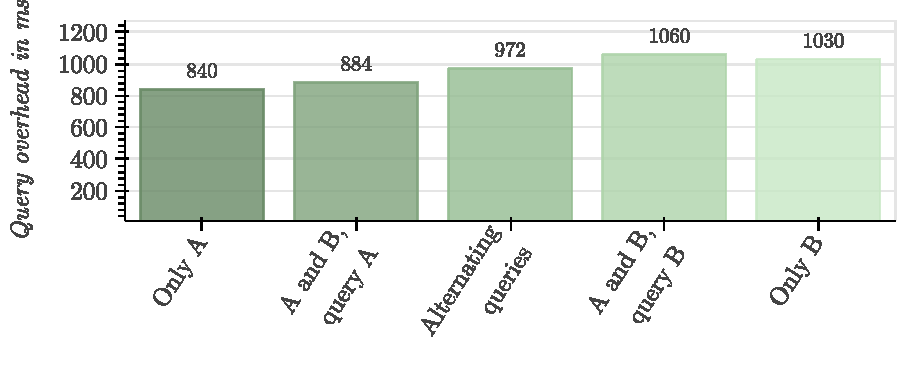
\includegraphics[width=\columnwidth]{multiple-attributes}
	\caption[Query overhead when using multiple attributes]{
		Query overhead when using multiple attributes.
		\emph{Only A} and \emph{Only B} index one attribute.
		\emph{A and B} indexes both attributes and then queries one of them.
		\emph{Alternating} indexes both attributes and runs half of the queries against \emph{A} and another half against \emph{B}.
	}%
	\label{figure:attributes}
\end{figure}
